\chapter{Admin}
Wesentlicher Bestandteil unseres Projektes war die Administrationsumgebung. Genauer musste eine Anwendung geschaffen werden, die dem jeweiligen Endanwender Navigationsdaten zur Verfügung stellt. Also eine Umgebung, die einen Upload für Kartenmaterial bereitstellt. Des weiteren muss die Administrationsanwendung Features besitzen um Routen zu definieren und Meta-Informationen zu besonderen Örtlichkeiten festhalten zu können. Die Meta-Informationen können durch Points of Interest (PoI) Informationen erweitert werden.\\
Im folgenden Abschnitt wird zunächst die allgemeine Struktur erläutert und anschließend liegt das Hauptaugenwerk auf der Benutzeroberfläche. Eine ausführliche Bedienungsanleitung der Administrationsumgebung ist im Anhang beigefügt.

\section{Allgemeine Struktur}
\subsection*{ASP.NET MVC 4}
Basis unserer Projektstruktur war das \textbf{ASP.NET MVC Framework}, welches ein Web Application Framework ist, und ein Model-View-Controller-Pattern implementiert.\\
Dies ermöglichte uns, eine Webanwendung zu entwickeln, bei der die Daten (\textit{Model}) gekapselt von der Ausgabe (\textit{View}) und dem \textit{Controller} vorliegen. Die \textit{View} repräsentiert unsere Daten und der \textit{Controller} reagiert auf Zustandsänderungen und ist sozusagen das Bindeglied oder die Schnittstelle zwischen \textit{View} und \textit{Model}.

\subsection{Model}
\subsubsection*{AccountModels}
Kapselt die benutzerspezifischen Daten in einem Model zur Authentifizierung von Benutzerprofilen. Dieses Model findet Verwendung beim Registrieren sowie beim LogIn- / LogOut-Verfahren.
\subsubsection*{AdminModels}
Model indem der MapName gekapselt vorliegt.
\subsubsection*{FloorViewModel}
Dieses Model enthält Daten zu einem Floor. FloorId, MapId und FloorImageFile sind diese Daten.
\subsubsection*{MapViewModel}
MapId und Name werden für die MapView in diesem Model gekapselt.

\subsection{View}
Die Views in unserem Projekt wurden in Views die den Account-, den Admin- und den Home-Bereich betreffen unterteilt.
\subsubsection*{Account}
Enthält html-Seiten zum registrieren, anmelden und verwalten den eigenen Benutzerprofils.
\subsubsection*{Admin}
Unter dieser Rubrik fallen die Webseiten, mit dem der Administrator Maps, Floors und Knoteninformationen zu einer Map hinzufügen kann. Sozusagen die Arbeitsoberfläche des Administrators.
\subsubsection*{Home}
Einstiegspunkt oder oberstes Element (Index) unserer Webseite.

\subsection{Controller}
\subsubsection*{HomeController}
Speziell für unser Projekt bedeutet es, dass wir drei Controller angelegt haben. Der Einstiegspunkt unserer Web-Anwendung ist der sogenannte \textit{HomeController}. Dies ist der Controller, der zum Zuge kommt, sofern die anderen beiden Controller eine Interaktion oder Controller-Aufrufe mit gewissen Parametern nicht unterstützen.
\subsubsection*{AccountController}
Der \textit{AccountController} verarbeitet die Ereignisse, die vom Registrierungs-, LogIn- und LogOut-Verhalten eines Benutzers ausgelöst werden. Im Fokus stehen hierbei die \textbf{HTTP GET-} und \textbf{HTTP POST-Methoden}, die von der Klasse \textit{AccountController} implementiert werden.
\subsubsection*{AdminController}
Der \textit{AdminController} reagiert auf Zustandsänderungen, die beim Anlegen, Bearbeiten und Löschen von Datenmaterial in Form von Karten oder Informationen (Meta-Informationen), ausgelöst werden.\\
Relevante Funktionen sind die Methoden zum erstellen und löschen von Maps und Floors.
Des weiteren werden über diesen Controller die Routeninformationen als Graph verarbeitet und in einer Datenbank gespeichert. Detailinformationen zu einem Knoten aus einem Graphen verarbeitet dieser Controller und speichert sie ab. Diese Detailinformationen ermöglichen besondere Orte als \textit{Points of Interest} zu kennzeichnen.

\section{Benutzeroberfläche}
Die Administrator Benutzeroberfläche ist über folgenden Link \\
\href{URL}{http://193.175.199.115/StudMapAdmin/} erreichbar.
\begin{figure}[H]
\centering
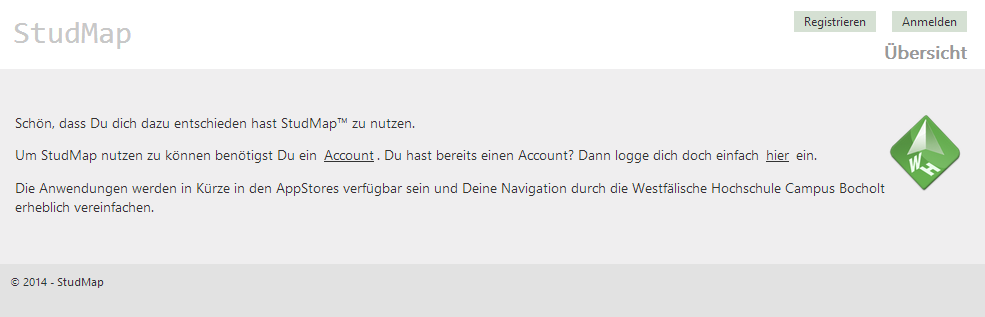
\includegraphics[width=\linewidth]{../Bilder/Admin/AdminHome}
\label{fig:AdminHome}
\end{figure}
Der Anwender enthält die Möglichkeit sich anzumelden oder sich zu registrieren.
\subsubsection*{Registrieren}
\href{URL}{http://193.175.199.115/StudMapAdmin/Account/Register}
\begin{figure}[H]
\centering
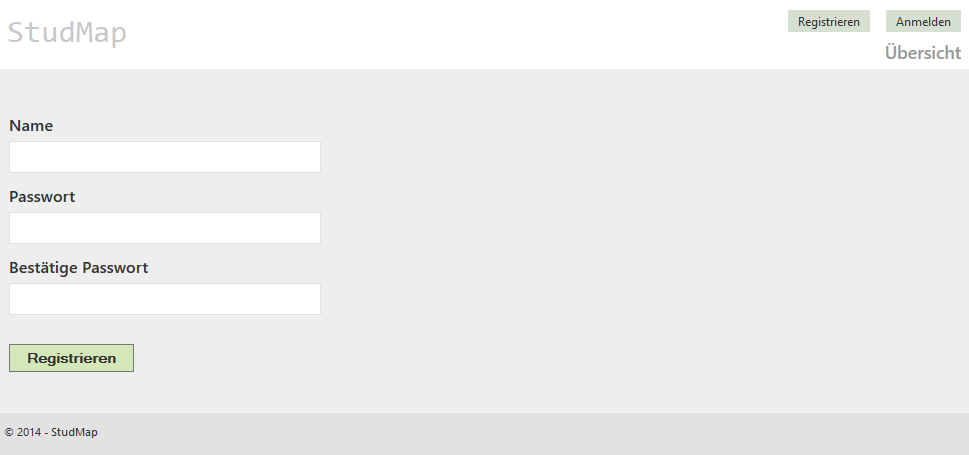
\includegraphics[width=\linewidth]{../Bilder/Admin/AdminRegistrierung}
\label{fig:AdminRegistrierung}
\end{figure}
\subsubsection*{Anmelden}
\href{URL}{http://193.175.199.115/StudMapAdmin/Account/Login}
\begin{figure}[H]
\centering
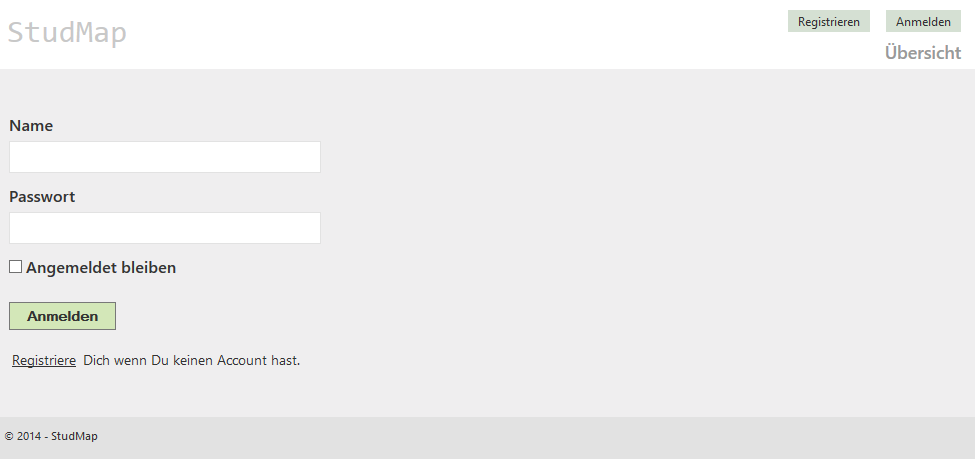
\includegraphics[width=\linewidth]{../Bilder/Admin/AdminAnmelden}
\label{fig:AdminAnmelden}
\end{figure}

\subsubsection*{Admin}
Den Einstiegspunkt zum verwalten von Maps finden Sie unter folgenden Link \\
\href{URL}{http://193.175.199.115/StudMapAdmin/Admin}. Er enthält eine Auflistung aktuell vorhandener Maps. Es  können neue Maps erstellt, bzw. vorhandene entfernt werden.
\begin{figure}[H]
\centering
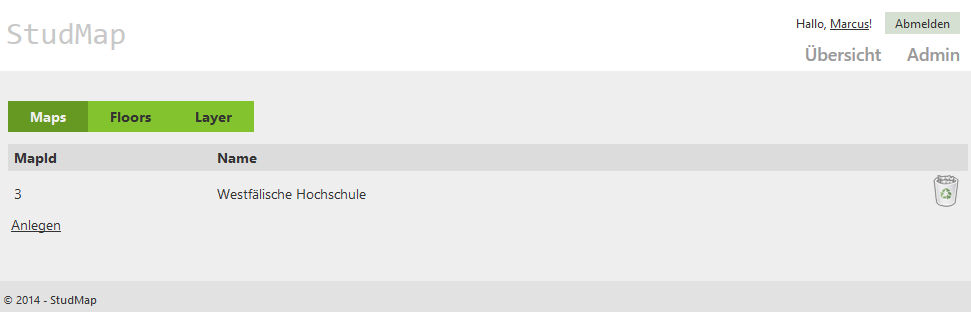
\includegraphics[width=\linewidth]{../Bilder/Admin/AdminMaps}
\label{fig:AdminMaps}
\end{figure}
Die Verwaltung der einzelnen Floors zu einer Map werden in der nachfolgenden Grafik gezeigt. Durch einen Klick auf \textit{Anlegen} kann eine neue Floor, mit der zugehörigen Kartengrundlage hinzugefügt werden.
\begin{figure}[H]
\centering
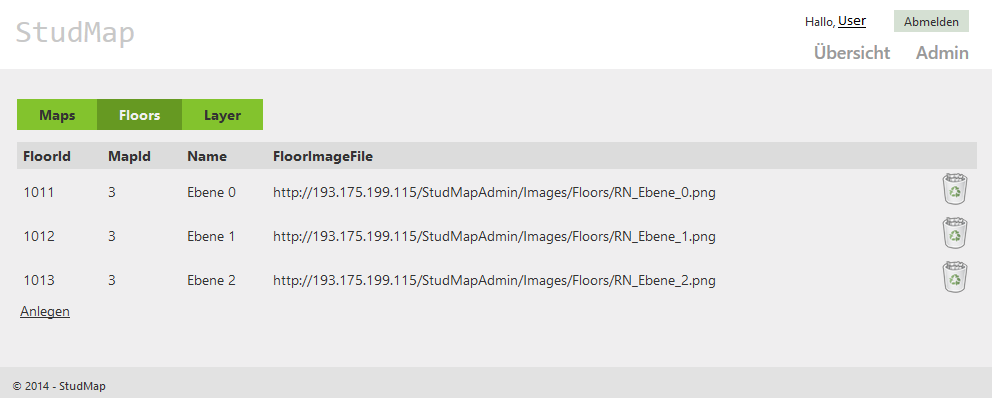
\includegraphics[width=\linewidth]{../Bilder/Admin/AdminFloors}
\label{fig:AdminFloors}
\end{figure}
Der Layer zeigt die Karte und einen gegebenenfalls erstellten Graphen mit Knoten und Kanten zu genau einem Floor an.
Durch Verwendung spezieller Features kann der Administrator hier einen Graphen erstellen und Knoteninformationen hinterlegen. Des weiteren besteht die Möglichkeit Knoten mit Knoten anderer Floors zu verknüpfen. Basis für eine ergonomische Navigation der Karte ist die JavaScript-Bibliothek D3.
\begin{figure}[H]
\centering
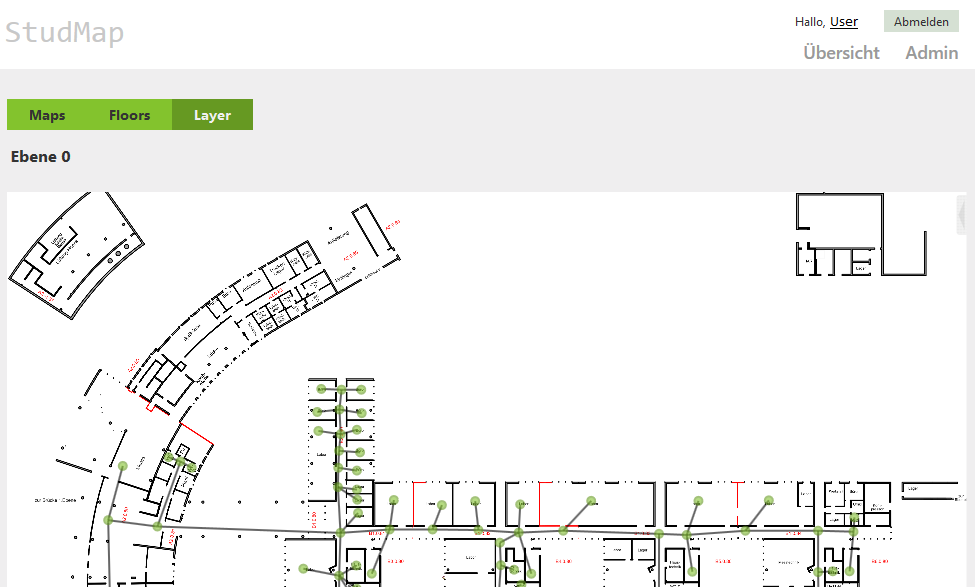
\includegraphics[width=\linewidth]{../Bilder/Admin/AdminLayer}
\label{fig:AdminLayer}
\end{figure}
\begin{figure}[H]
\centering
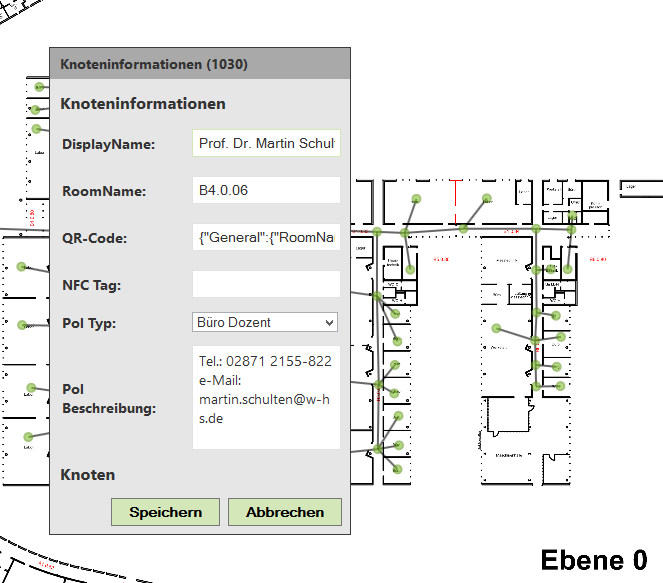
\includegraphics[width=\linewidth]{../Bilder/Admin/AdminNodeInfo}
\label{fig:AdminNodeInfo}
\end{figure}
Über den Button \textit{Abmelden} gelangen Sie zum Index unserer Webseite zurück.

\section{Admin Spezifisches}
\subsection*{Neuen Benutzer mit Administrator Rechten versehen}
\label{Administrator Rechte versehen}
Nachdem ein neuer Benutzer die Registratur erfolgreich abgeschlossen hat, ist dieser im Benutzerprofil noch nicht als Administrator gekennzeichnet. Derzeit ist es so, dass ein Datenbankadministrator in der Tabelle \textit{webpages\_UsersInRoles} den Eintrag von 1 für Users auf 2 für Admins abändern muss. Nur Admins haben die Rechte Maps und Floors zu erstellen, sowie das Kartenmateral mit Metainformationen zu bereichern.
\subsection*{ELMAH}
Als Logging Werkzeug haben wir das auf der .NET Plattform sehr verbreitete und OpenSource Tool \textit{ELMAH} eingesetzt. \textit{ELMAH}\footnote{ELMAH steht für "Error Logging Modules and Handlers"} loggt auftretende Fehler und Exceptions. Nach kurzem Installationsaufwand und Konfiguration einer Datenbank, in der die Fehler gespeichert werden, kann das Tool bereits genutzt werden. Genaue Installationsanleitungen findet Sie zu genüge im Internet.
\href{URL}{http://blog.thomasbandt.de/39/2380/de/blog/elmah-mit-aspnet-mvc-nutzen-und-fehler-loggen.html} 

% für den Anhang 
\section{Admin-Bedienungsanleitung}
\subsection*{Registrieren}
\begin{enumerate}
\item Aufruf der Webseite: \href{URL}{http://193.175.199.115/StudMapAdmin/Account/Register}.
		\begin{figure}[H]
		\centering
		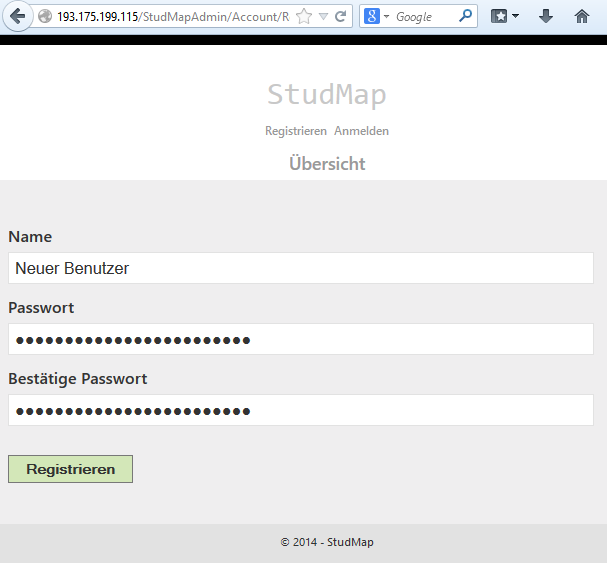
\includegraphics[width=0.7\linewidth]{../Bilder/Admin/AnleitungRegistratur1}
		\label{fig:AnleitungRegistratur1}
		\end{figure}
\item Button \textit{Registrieren} betätigen.
\item Datenbankadministrator muss den \nameref{Administrator Rechte versehen}.
\end{enumerate}

\subsection*{LogIn / LogOut}
\begin{enumerate}
\item Aufruf der Webseite: \href{URL}{http://193.175.199.115/StudMapAdmin/Account/Login}.
\item Benutzername und Passwort eingeben.
\item Button \textit{Anmelden} betätigen.
\item Sie können sich jederzeit über den Button \textit{Abmelden} ausloggen.
\end{enumerate}

\subsection*{Passwort ändern}
\begin{enumerate}
\item Aufruf der Webseite: \href{URL}{http://193.175.199.115/StudMapAdmin/Account/Manage} oder auf eigenen Benutzernamen klicken.
\item Aktuelles Kennwort und gewünschtes neues Kennwort eingeben. Dieses zusätzlich bestätigen.
\item Button \textit{Passwort ändern} betätigen.
\end{enumerate}

\subsection*{Neue Map anlegen}
\begin{enumerate}
\item Aufruf der Webseite: \href{URL}{http://193.175.199.115/StudMapAdmin/Admin/CreateMap} oder auf der Admin Seite auf \textit{anlegen} klicken.
\item Anschließend Map-Namen eingeben und bestätigen.
\item Map kann über das Papierkorb-Symbol gelöscht werden.
\end{enumerate}

\subsection*{Neuen Floor anlegen}
\begin{enumerate}
\item Aufruf der Webseite: \href{URL}{http://193.175.199.115/StudMapAdmin/Admin}. 
\item Anschließend auf den Map-Namen klicken.
\item Über den Button \textit{Anlegen} gelangen Sie nun zur Seite auf der Sie einen Floor hinzufügen können.
\item Den Eintrag MapId wird automatisch übernommen.
\item Sie geben den Floor-Namen ein und ergänzen einen Link zu Ihrer Kartengrundlage \footnote{Bevorzugtes Format der Karte sind PDF und PNG Files.}.
\item Abschließend betätigen Sie den Button \textit{Anlegen}.
\end{enumerate}

\subsection*{Menühandhabung des Layers}
\begin{enumerate}
\item Aufruf der Webseite: \href{URL}{http://193.175.199.115/StudMapAdmin/Admin}. 
\item Anschließend auf den Map-Namen klicken.
\item Dann auf den Floor-Namen klicken.
\item Sie können über das Mausrad in die Karte, bzw. aus der Karte hinaus zoomen und das Kartenwerk verschieben indem Sie die linke Maustaste gedrückt halten und die Maus hin und her bewegen.
\item Des weiteren können Sie folgende Features ausüben, um die Karte mit Meta-Informationen zu ergänzen:
	\begin{itemize}
	\item \nameref{Knoten anlegen}
	\item \nameref{Kanten anlegen}
	\item \nameref{Knoten loeschen}
	\item \nameref{Knoteninformationen hinterlegen}
	\item \nameref{Knoten mit Knoten auf anderem Floor verbinden}
	\end{itemize} 
\end{enumerate}

\subsubsection*{Knoten anlegen}
\label{Knoten anlegen}
\begin{enumerate}
\item Sie befinden sich auf der Layer Webseite und haben das Kartenwerk vor Augen.
\item Sie zoomen an die entsprechende Stelle an der Sie einen Knoten erzeugen möchten mit dem Mausrad.
\item Dann betätigen Sie in Kombination mit der \textit{Strg-Taste} die \textit{linke Maustaste}.
\item Abschließend müssen Sie den Button \textit{Speichern} betätigen, den Sie sehen müssten wenn sie komplett raus gezoomt haben.
\end{enumerate}
\subsubsection*{Kanten anlegen}
\label{Kanten anlegen}
\begin{enumerate}
\item Sie befinden sich auf der Layer Webseite und haben das Kartenwerk vor Augen.
\item Zwei Knoten werden mit einander verbunden, indem Sie zuerst einen der beiden Knoten mit einem einfachen Klick mit der \textit{linken Maustaste} markieren.
\item Anschließend navigieren Sie zum zweiten Knoten. Durch einen Klick mit der \textit{linken Maustaste} werden beide Knoten mit einer Kante miteinander verbunden.
\item Speichern Sie Ihr Ergebnis über den entsprechenden Button ab.
\end{enumerate}
\subsubsection*{Knoten löschen}
\label{Knoten loeschen}
\begin{enumerate}
\item Sie befinden sich auf der Layer Webseite und haben das Kartenwerk vor Augen.
\item Sie zoomen zu den Knoten, den es zu entfernen gilt.
\item Markieren Sie den Knoten mit der \textit{linken Maustaste}.
\item Betätigen Sie die Taste \textit{Entf} auf Ihrer Tastatur. Der Knoten und anliegende Kanten sind entfernt worden.
\item Vergessen Sie nicht den aktuell vorliegenden Graphen zu speichern.
\end{enumerate}
\subsubsection*{Knoteninformationen hinterlegen}
\label{Knoteninformationen hinterlegen}
\begin{enumerate}
\item Sie befinden sich auf der Layer Webseite und haben das Kartenwerk vor Augen.
\item Durch einen einfachen Klick mit der \textit{rechten Maustaste} erhalten Sie gezieltere Informationen zum Knoten.
		\begin{figure}[H]
		\centering
		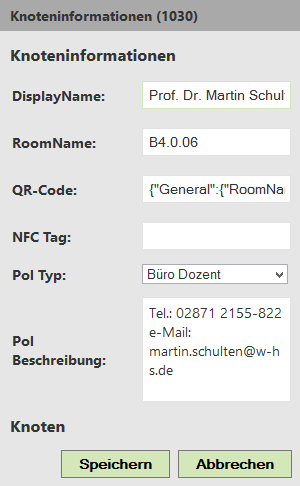
\includegraphics[width=0.3\linewidth]{../Bilder/Admin/AnleitungKnoteninformationen1}
		\label{fig:AnleitungKnoteninformationen1}
		\end{figure}
\item Sie können die den Knoten um Informationen erweitern, indem Sie entsprechende Vermerke in den Textboxen vornehmen.
	\begin{itemize}
	\item Display Name: Sprechender Name des Raumes
	\item RoomName: Einmalige Raumbezeichnung
	\item QR-Code: Von uns automatisierter QR-Code für diesen Raum
	\item NFC-Tag: NFC-Tag ID für diesen Raum
	\item PoI-Type: Art des Raumes, z.B. Labor
	\item PoI-Beschreibung: Informationen die diesen Raum genauer beschreiben oder die Sie diesem Knoten zusätzlich hinterlegen wollen.
	\end{itemize}
\item Die Knoten Id und die genauen Koordinaten des Knotens, in Prozent, werden angezeigt nachdem Sie auf das Stichwort \textbf{Knoten} mit der Maus navigieren.
\item Info: Ergänzen Sie einen Knoten um Informationen erst, nachdem Sie den Graphen gespeichert haben. Ansonsten gehe Ihre Eingaben verloren.
\end{enumerate}
\subsubsection*{Knoten mit Knoten auf anderem Floor verbinden}
\label{Knoten mit Knoten auf anderem Floor verbinden}
\begin{enumerate}
\item Sie befinden sich auf der Layer Webseite und haben das Kartenwerk vor Augen.
\item Zuerst benötigen Sie die Knoten Id's, mit den Sie Ihren Knoten verbinden möchten. Also müssen Sie sich möglicherweise die Id eines Knotens einer anderen Floor notieren.
\item Betätigen Sie die \textit{Shift-Taste} + \textit{Linke Maustaste} auf den Knoten:
		\begin{figure}[H]
		\centering
		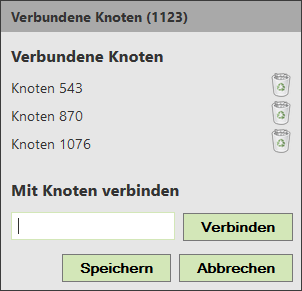
\includegraphics[width=0.3\linewidth]{../Bilder/Admin/AnleitungKnotenMiteinanderVerbinden}
		\label{fig:AnleitungKnotenMiteinanderVerbinden}
		\end{figure}
\item Tragen Sie die Id ein.
\item Drücken Sie den Button \textit{Verbinden}
\item Abschließend betätigen Sie den Button \textit{Speichern} und zwei Knoten wurden über diesen Weg miteinander verbunden.
\end{enumerate}

% TODOS:
% - Funktionsweise (Knoten über zwei Ebenen miteinander verbinden)
% - UI Aspekte (x)
% - MVC Web Zeug... (x)
% - Verweis auf Anhang für Bedienungsanleitung / Installationsanleitung